%   Filename    : chapter_4.tex 
\section*{Chapter 4}
\section{Results and Discussions}
\subsection{Data Gathered}

The researchers have contacted their resource person Prof. Dimzon on her collection of folk narratives. She gave a Terminal Report \citeA{dimzonmyths} on her completed project on collecting myths and legends from Western Visayas. It listed a total of 189 stories, 28 being myths, 161 being legends and 9 categorized as others. Each folk narrative has already been categorized into their respective types, including etiological legends, non-etiological legends, and others. Below is a list of the different types of folk narratives collected, their subtypes, and their count.

\begin{enumerate}[label=\Roman*.]
\item Myths: 28
    \item Legends: 161
    \begin{enumerate} [label=\Alph*.]
        \item Etiological Legends: 69
        \begin{enumerate}[label=\roman*.]
            \item How Legends: 59
            \begin{enumerate}[label=\alph*.]
                \item Origin of Animals: 14
                \item Origin of plants and forms of plant life: 4
                \item How places and things got their names: 41
            \end{enumerate}
        \end{enumerate}
        \item NonEtiological Legends: 83
            \begin{enumerate}[label=\roman*.]
                \item Heroic Legends - great men, culture heroes: 18
                \item Religious/Saints Legends: 9
                \item Legends on Supernatural/Enchanted Beings: 56
            \end{enumerate}
        \item Others: 9
    \end{enumerate}
\end{enumerate}

However, some of these folk narratives were out of scope for the special project as it focuses purely on stories from Panay Island only. Below is the number of stories after filtering for Panayanon specific narratives. In summary, there were 21 myths, 108 legends, and 7 categorized as others.

\begin{enumerate}[label=\Roman*.]
\item Myths: 21
    \item Legends: 108
    \begin{enumerate} [label=\Alph*.]
        \item Etiological Legends: 43
        \begin{enumerate}[label=\roman*.]
            \item How Legends: 36
            \begin{enumerate}[label=\alph*.]
                \item Origin of Animals: 9
                \item Origin of plants and forms of plant life: 3
                \item How places and things got their names: 24
            \end{enumerate}
        \end{enumerate}
        \item NonEtiological Legends: 64
            \begin{enumerate}[label=\roman*.]
                \item Heroic Legends - great men, culture heroes: 11
                \item Religious/Saints Legends: 9
                \item Legends on Supernatural/Enchanted Beings: 44
            \end{enumerate}
        \item Others: 7
    \end{enumerate}
\end{enumerate}

\subsection{New Classes}
    As per consultation with Mrs. Dimzon, the following classes were added to expand on the original ontology.

\begin{table}[h]
    \centering
    \begin{tabular}{|l|l|l|}
        \hline
        \textbf{Class} & \textbf{Subclass} & \textbf{Subsubclass} \\ \hline
        GeographicFeature &  &  \\ \hline
         & Landform &  \\ \hline
         &  & Mountain \\ \hline
         &  & Hill \\ \hline
         &  & Forest \\ \hline
         &  & Forest \\ \hline
         &  & Island \\ \hline
         &  & Volcano \\ \hline
         & BodyOfWater &  \\ \hline
         &  & River \\ \hline
         &  & Sea \\ \hline
         &  & Ocean \\ \hline
         &  & Lake \\ \hline
        Language &  &  \\ \hline
         &   Hiligaynon & \\ \hline
         &   Kinaray-a & \\ \hline
         &   Akeanon & \\ \hline
        \end{tabular}
    \caption{Hierarchy of Classes, Subclasses, and Subsubclasses}
    \label{tab:class-subclass}
\end{table}

Figure \ref{fig:class hierarchy} presents the class hierarchy of the objects in the original ontology as presented in Protege. Classes are categories or types of things in the ontology, representing a group of objects or individuals that share common characteristics. Instances of these classes are called individuals in Protege, representing a specific thing that belongs to the class. 

\begin{figure}[H]
    \centering
    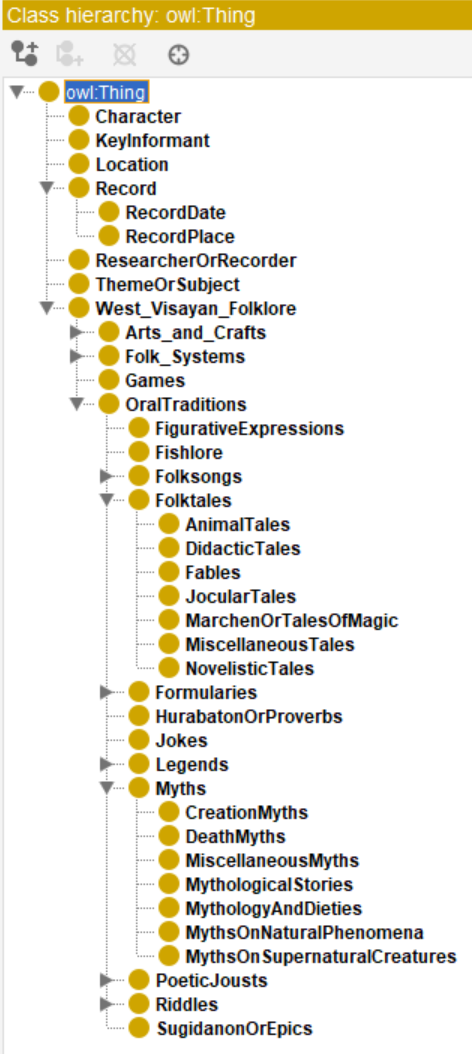
\includegraphics[width=0.5\linewidth]{figures/Class Hierarchy of Original Ontology.png}
    \caption{Class Hierarchy of Original Ontology}
    \label{fig:class hierarchy}
\end{figure}

With the newly introduced classes, \ref{fig:class hierarchy enhanced} presents the class hierarchy of the objects in the enhanced ontology as presented in Protege.

\begin{figure}[H]
    \centering
    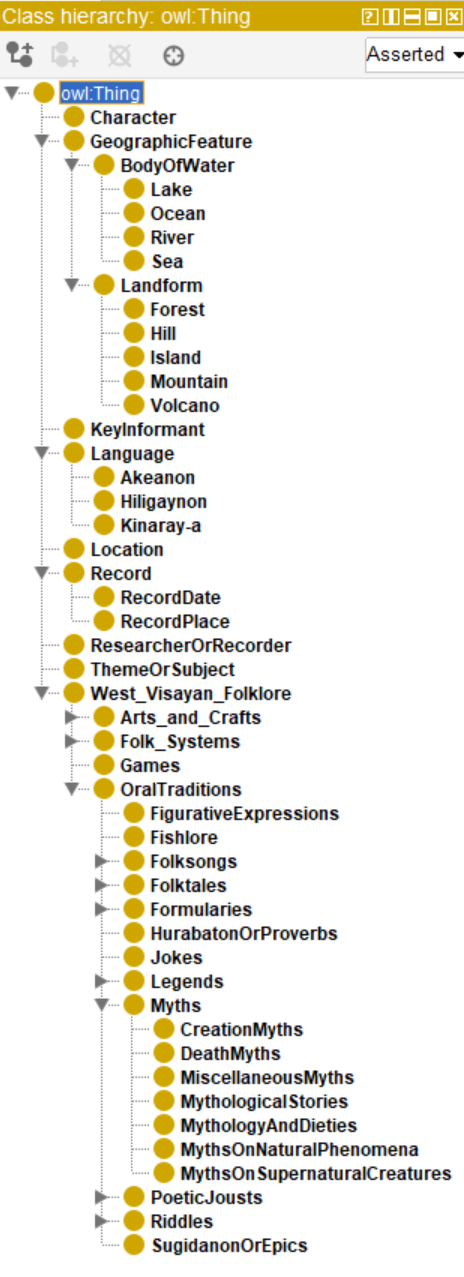
\includegraphics[width=0.5\linewidth]{figures/Class Hierarchy of Enhanced Ontology.png}
    \caption{Class Hierarchy of Enhanced Ontology}
    \label{fig:class hierarchy enhanced}
\end{figure}

Figure \ref{fig:object property hierarchy} presents the hierarchy of the object properties in the original ontology as presented in Protege. Object properties define relationships between two individuals in the ontology, and are used to link classes or instances. In the ontology enhancement phase, the researchers will introduce new object properties to accommodate the new classes.

\begin{figure}[H]
    \centering
    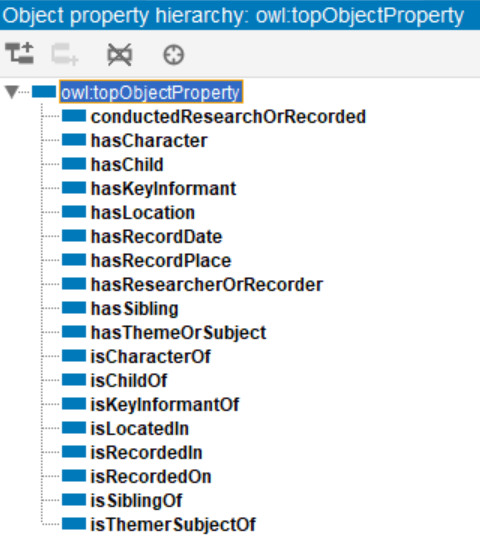
\includegraphics[width=0.5\linewidth]{figures/Object Property Hierarchy of Original Ontology.png}
    \caption{Object Property Hierarchy of Original Ontology}
    \label{fig:object property hierarchy}
\end{figure}

With the newly introduced classes, \ref{fig:object property hierarchy enhanced} presents the the hierarchy of the object properties in the enhanced ontology as presented in Protege.

\begin{figure}[H]
    \centering
    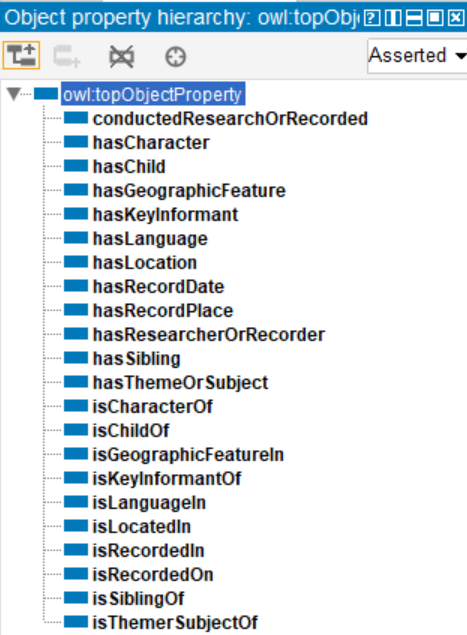
\includegraphics[width=0.5\linewidth]{figures/Object Property Hierarchy of Enhanced Ontology.png}
    \caption{Object Property Hierarchy of Original Ontology}
    \label{fig:object property hierarchy enhanced}
\end{figure}

Figure \ref{fig:data property hierarchy} presents the hierarchy of the data properties in the original ontology as presented in Protege. Data properties define relationships between an individual and a literal value, such as a string, number, or date. There was no need to add new data properties with the introduction of the new classes.

\begin{figure}[H]
    \centering
    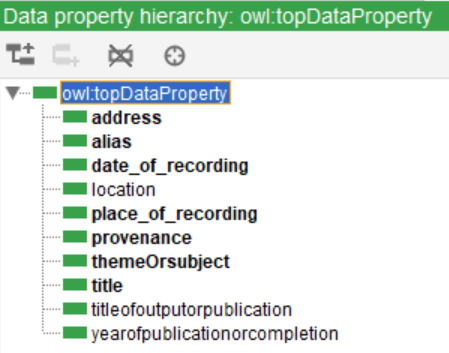
\includegraphics[width=0.5\linewidth]{figures/Data Property Hierarchy of Original Ontology.png}
    \caption{Data Property Hierarchy of Original Ontology}
    \label{fig:data property hierarchy}
\end{figure}

\FloatBarrier